\documentclass[a4paper,11pt]{report}
\usepackage{chuan_math_gkt}
\usetikzlibrary{angles,quotes,intersections,patterns,decorations.pathreplacing}
\chuanexamsetup

\begin{document}
\examfontsize

\examsecret{绝密$\bigstar$启用前}

\examtitle{2023年普通高等学校招生全国统一考试（北京卷）}{数\quad 学}

\noticetitle
\begin{examnotice}
\item 答卷前，考生务必将自己的姓名、准考证号填写在答题卡上。
\item 回答选择题时，选出每小题的答案后，用铅笔把答题卡上对应题目的答案标号涂黑。如需改动，用橡皮擦干净后，再选涂其他答案标号。回答非选择题时，将答案写在答题卡上。写在本试卷上无效。
\item 考试结束后，将本试卷和答题卡一并交回。
\end{examnotice}


\examsection{一、选择题：本题共10小题，每小题4分，共40分。在每小题给出的四个选项中，只有一项是符合题目要求的。}
\begin{examquestions}
\item 已知集合 $M=\{x\mid x+2\geq0\}$，$N=\{x\mid x-1<0\}$，则 $M\cap N=$
\fourchoices{$\{x\mid -2\leq x<1\}$}{$\{x\mid -2<x\leq1\}$}{$\{x\mid x\geq-2\}$}{$\{x\mid x<1\}$}
\item 在复平面内，复数 $z$ 对应的点的坐标是 $(-1,\sqrt3)$，则 $z$ 的共轭复数 $\overline z=$
\fourchoices{$1+\sqrt3\mathrm{i}$}{$1-\sqrt3\mathrm{i}$}{$-1+\sqrt3\mathrm{i}$}{$-1-\sqrt3\mathrm{i}$}
\item 已知向量 $\vec a,\vec b$ 满足 $\vec a+\vec b=(2,3)$，$\vec a-\vec b=(-2,1)$，则 $|\vec a|^2-|\vec b|^2=$
\fourchoices{$-2$}{$-1$}{$0$}{$1$}
\item 下列函数中，在区间 $(0,+\infty)$ 上单调递增的是
\fourchoices{$f(x)=-\ln x$}{$f(x)=\dfrac1{2^x}$}{$f(x)=-\dfrac1x$}{$f(x)=3^{x-1}$}
\item $(2x-\dfrac1x)^5$ 的展开式中 $x$ 的系数为
\fourchoices{$-80$}{$-40$}{$40$}{$80$}
\item 已知抛物线 $C:y^2=8x$ 的焦点为 $F$，点 $M$ 在 $C$ 上. 若 $M$ 到直线 $x=-3$ 的距离为 $5$，则 $|MF|=$
\fourchoices{$7$}{$6$}{$5$}{$4$}
\item 在 $\triangle ABC$ 中，$(a+c)(\sin A-\sin C)=b(\sin A-\sin B)$，则 $\angle C=$
\fourchoices{$\dfrac\pi6$}{$\dfrac\pi3$}{$\dfrac{2\pi}3$}{$\dfrac{5\pi}6$}
\newpage
\item 若 $xy\ne0$，则“$x+y=0$”是“$\dfrac{y}{x}+\dfrac{x}{y}=-2$”的
\twochoices{充分不必要条件}{必要不充分条件}{充要条件}{既不充分也不必要条件}
\item 坡屋顶是我国传统建筑造型之一，蕴含着丰富的数学元素. 安装灯带可以勾勒出建筑轮廓，展现造型之美. 如图，某坡屋顶可视为一个五面体，其中两个面是全等的等腰梯形，两个面是全等的等腰三角形. 若 $AB=25\mathrm m$，$BC=AD=10\mathrm m$，且等腰梯形所在的平面、等腰三角形所在的平面与平面 $ABCD$ 的夹角的正切值均为 $\dfrac{\sqrt{14}}5$，则该五面体的所有棱长之和为
\begin{tightcenter}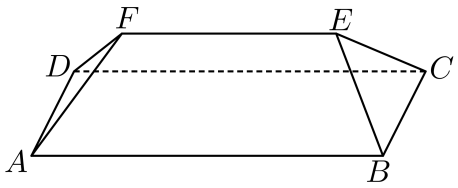
\includegraphics[width=5.0cm]{figures/2023_bj_q9.png}\end{tightcenter}
\fourchoices{$60\mathrm m$}{$65\mathrm m$}{$70\mathrm m$}{$75\mathrm m$}
\item 已知数列 $\{a_n\}$ 满足 $a_{n+1}=\dfrac{a_n+3}{a_n+1}$，则
\onechoices{当 $a_1=3$ 时，$\{a_n\}$ 为递减数列，且存在常数 $M\leq0$，使得 $a_n>M$ 恒成立}{当 $a_1=5$ 时，$\{a_n\}$ 为递增数列，且存在常数 $M\leq6$，使得 $a_n<M$ 恒成立}{当 $a_1=7$ 时，$\{a_n\}$ 为递减数列，且存在常数 $M>6$，使得 $a_n>M$ 恒成立}{当 $a_1=9$ 时，$\{a_n\}$ 为递增数列，且存在常数 $M>0$，使得 $a_n<M$ 恒成立}
\end{examquestions}

\examsection{二、填空题：本题共5小题，每小题5分，共25分。}
\begin{examquestions}[start=11]
\item 已知函数 $f(x)=4^x+\log_2 x$，则 $f\left(\dfrac12\right)=$\blank.
\item 已知双曲线 $C$ 的焦点为 $(-2,0)$ 和 $(2,0)$，离心率为 $\sqrt2$，则 $C$ 的方程为\blank.
\item 已知命题 $p$：若 $\alpha,\beta$ 为第一象限角，且 $\alpha>\beta$，则 $\tan\alpha>\tan\beta$. 能说明 $p$ 为假命题的一组 $\alpha,\beta$ 的值为 $\alpha=$\blank，$\beta=$\blank.
\item 我国度量衡的发展有着悠久的历史，战国时期就已经出现了类似于砝码的、用来测量物体质量的“环权”. 已知 $9$ 枚环权的质量（单位：铢）从小到大构成项数为 $9$ 的数列 $\{a_n\}$，该数列的前 $3$ 项成等差数列，后 $7$ 项成等比数列，且 $a_1=1$，$a_5=12$，$a_9=192$，则 $a_7=$\blank；数列 $\{a_n\}$ 所有项的和为\blank.
\newpage
\item 设 $a>0$，函数 $f(x)=\linsys{x+2,\quad x<-a,\\\sqrt{a^2-x^2},\quad -a\leq x\leq a,\\-\sqrt{x-1},\quad x>a}$. 给出下列四个结论：

①$f(x)$ 在区间 $(a-1,+\infty)$ 上单调递减；

②当 $a\geq1$ 时，$f(x)$ 存在最大值；

③设 $M(x_1,f(x_1))(x_1\leq a)$，$N(x_2,f(x_2))(x_2>a)$，则 $|MN|>1$；

④设 $P(x_3,f(x_3))(x_3<-a)$，$Q(x_4,f(x_4))(x_4\geq -a)$. 若 $|PQ|$ 存在最小值，则 $a$ 的取值范围是 $\left(0,\dfrac12\right]$. 

其中所有正确结论的序号是\blank.
\end{examquestions}

\examsection{三、解答题：本题共6小题，共85分。解答应写出文字说明、证明过程或演算步骤。}
\begin{examanswers}[start=16]
\item（13分）

如图，在三棱锥 $P-ABC$ 中，$PA\perp$ 平面 $ABC$，$PA=AB=BC=1$，$PC=\sqrt3$.

\noindent\begin{minipage}[t]{0.62\linewidth}
（1）求证：$BC\perp$ 平面 $PAB$；

（2）求二面角 $A-PC-B$ 的大小.
\end{minipage}\hfill
\begin{minipage}[t]{0.25\linewidth}
\vspace{-1.0em}\centering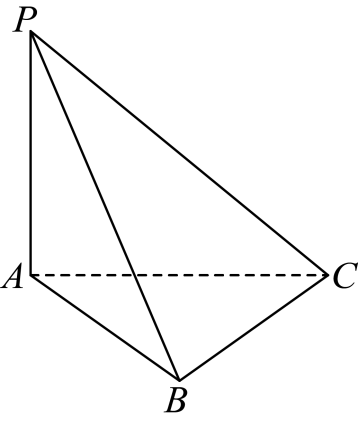
\includegraphics[width=\linewidth]{figures/2023_bj_q16.png}
\end{minipage}
\item（13分）

设函数 $f(x)=\sin\omega x\cos\varphi+\cos\omega x\sin\varphi\left(\omega>0,|\varphi|<\dfrac\pi2\right)$.

（1）若 $f(0)=-\dfrac{\sqrt3}{2}$，求 $\varphi$ 的值.

（2）已知 $f(x)$ 在区间 $\left[-\dfrac\pi3,\dfrac{2\pi}3\right]$ 上单调递增，$f\left(\dfrac{2\pi}3\right)=1$，再从条件①、条件②、条件③这三个条件中选择一个作为已知，使函数 $f(x)$ 存在，求 $\omega,\varphi$ 的值.

条件①：$f\left(\dfrac\pi3\right)=\sqrt2$；条件②：$f\left(-\dfrac\pi3\right)=-1$；条件③：$f(x)$ 在区间 $\left[-\dfrac\pi2,-\dfrac\pi3\right]$ 上单调递减.
\newpage
\item（14分）

为研究某种农产品价格变化的规律，收集得到了该农产品连续 $40$ 天的价格变化数据，如下表所示. 在描述价格变化时，用“$+$”表示“上涨”，用“$-$”表示“下跌”，用“$0$”表示“不变”.
\begin{tightcenter}\small
\begin{tabular}{c|c}
\hline
时段 & {价格变化}\\ \hline
第1天到第20天  & $-$  $+$  $+$  $0$  $-$  $-$  $-$  $+$  $+$  $0$  $+$  $0$  $-$  $-$  $+$  $-$  $+$  $0$  $0$  $+$\\
第21天到第40天 & $0$  $+$  $+$  $0$  $-$  $-$  $-$  $+$  $+$  $0$  $+$  $0$  $+$  $-$  $-$  $-$  $+$  $0$  $-$  $+$\\ \hline
\end{tabular}
\end{tightcenter}
用频率估计概率.

（1）试估计该农产品价格“上涨”的概率；

（2）假设该农产品每天的价格变化是相互独立的. 在未来的日子里任取 $4$ 天，试估计该农产品价格在这 $4$ 天中 $2$ 天“上涨”、$1$ 天“下跌”、$1$ 天“不变”的概率；

（3）假设该农产品每天的价格变化只受前一天价格变化的影响. 判断第 $41$ 天该农产品价格“上涨”“下跌”和“不变”的概率估计值哪个最大.（结论不要求证明）
\item（15分）

已知椭圆 $E:\dfrac{x^2}{a^2}+\dfrac{y^2}{b^2}=1(a>b>0)$ 离心率为 $\dfrac{\sqrt5}{3}$，$A,C$ 分别是 $E$ 的上、下顶点，$B,D$ 分别是 $E$ 的左、右顶点，$|AC|=4$.

（1）求 $E$ 的方程；

（2）设 $P$ 为第一象限内 $E$ 上的动点，直线 $PD$ 与直线 $BC$ 交于 $M$，直线 $PA$ 与直线 $y=-2$ 交于点 $N$. 求证：$MN\parallel CD$.
\item（15分）

设函数 $f(x)=x-x^3e^{ax+b}$，曲线 $y=f(x)$ 在点 $(1,f(1))$ 处的切线方程为 $y=-x+1$.

（1）求 $a,b$ 的值；

（2）设函数 $g(x)=f'(x)$，求 $g(x)$ 的单调区间；

（3）求 $f(x)$ 的极值点个数.
\newpage
\item（15分）

已知数列 $\{a_n\},\{b_n\}$ 的项数均为 $m(m>2)$，且 $a_n,b_n\in\{1,2,\cdots,m\}$，$\{a_n\},\{b_n\}$ 的前 $n$ 项和分别为 $A_n,B_n$，并规定 $A_0=B_0=0$. 对于 $k\in\{0,1,2,\cdots,m\}$，定义 $r_k=\max\{i\mid B_i\leq A_k,i\in\{0,1,2,\cdots,m\}\}$，其中 $\max M$ 表示数集 $M$ 中最大的数.

（1）若 $a_1=2,a_2=1,a_3=3,b_1=1,b_2=3,b_3=3$，求 $r_0,r_1,r_2,r_3$ 的值；

（2）若 $a_1\geq b_1$，且 $2r_j\leq r_{j+1}+r_{j-1}$，$j=1,2,\cdots,m-1$，求 $r_n$；

（3）证明：存在 $p,q,s,t\in\{0,1,2,\cdots,m\}$，满足 $p>q,s>t$，使得 $A_p+B_t=A_q+B_s$.
\end{examanswers}

\end{document}
